\chapter{Dataset e protocollo di validazione}
\label{chap:dataset}

Per confrontare i classificatori classici e ibridi, i modelli devono
essere valutati sugli stessi esempi. Questo capitolo descrive la
costruzione del dataset, dalla selezione del catalogo alle partizioni
di training, validation e test. Sono riportati i controlli usati per
garantire l'appaiamento e i limiti del campione selezionato.

Il dataset finale comprende \(5\,628\) immagini, suddivise in tre classi
bilanciate: galassie ellittiche, galassie spirali e sistemi classificati
come \emph{merger}.
A partire da questo insieme si definiscono
un problema binario, limitato alle ellittiche e alle spirali, e un
problema a tre classi, che include anche i merger. L’introduzione di
questi ultimi consente di valutare i modelli in uno scenario di
maggiore complessità morfologica, verificando se le differenze tra
classificatori classici e quantistici emergano più chiaramente
rispetto al caso binario. La valutazione si basa su dieci
ripetizioni di un holdout stratificato. Per ciascuna ripetizione
vengono costruiti sottoinsiemi stratificati del training set, al fine di
analizzare l’impatto della disponibilità dei dati.

\section{Provenienza dei dati e popolazione selezionata}
\label{sec:provenienza}

Le immagini e i metadati provengono dai servizi dello Sloan Digital Sky
Survey (SDSS), utilizzati attraverso la Data Release 17
(DR17)~\cite{abdurrouf2022dr17}. Le informazioni morfologiche sono quelle
di Galaxy Zoo presenti nella tabella \texttt{zooSpec}: il servizio di accesso
è DR17, ma ciò non implica che le classificazioni morfologiche siano state
prodotte originariamente per questa release. Galaxy Zoo raccoglie
classificazioni visuali collaborative, successivamente sintetizzate in
frazioni di voto e indicatori morfologici~\cite{lintott2011galaxyzoo}.

L'estrazione del catalogo è stata effettuata mediante una query CasJobs
che collega \texttt{PhotoObj}, \texttt{zooSpec} e \texttt{SpecObj}. Sono
richiesti il flag fotometrico \texttt{clean=1}, la classificazione
\texttt{type=3}, una magnitudine nella banda \(g\) compresa tra \(14\) e
\(17{,}5\) e un redshift compreso tra \(0{,}005\) e \(0{,}1\).
La query, riportata nell'\cref{app:query}, usa l'operatore
\texttt{BETWEEN}, che include gli estremi; il successivo controllo locale
sul redshift applica invece \(0{,}005<z<0{,}1\).

Il file esportato conserva identificativo dell'oggetto, ascensione retta,
declinazione, redshift e tre indicatori morfologici. Non conserva invece
le colonne \texttt{clean}, \texttt{type} e \(g\). I relativi vincoli sono
quindi documentati dalla query di estrazione, ma non possono essere
verificati nuovamente a partire dal solo CSV locale. Questa distinzione
separa la provenienza documentata dai controlli effettivamente ripetibili
sugli artefatti distribuiti.

La popolazione risultante non costituisce un campione indiscriminato di
tutte le galassie SDSS: disponibilità spettroscopica, intervallo di
magnitudine, redshift e selezione morfologica ne delimitano il campo di
validità. Le prestazioni misurate nella tesi si riferiscono a questa
popolazione selezionata.

\section{Assegnazione delle etichette}
\label{sec:etichette}

Per ellittiche e spirali vengono utilizzati rispettivamente
\texttt{p\_el\_debiased} e \texttt{p\_cs\_debiased}; per i merger viene
utilizzato \texttt{p\_mg}. Le prime due quantità includono una correzione
dei bias osservativi nella classificazione, mentre l'indicatore merger
ha una diversa origine nella struttura dei voti. Non è quindi opportuno
interpretare le tre soglie come livelli omogenei di probabilità calibrata
o come garanzie di correttezza della singola etichetta. Il ruolo delle
classificazioni Galaxy Zoo e dell'indicatore di fusione è discusso nei
lavori di rilascio e di selezione dei sistemi interagenti
\cite{lintott2011galaxyzoo,darg2010mergers}.

Le soglie operative sono riportate nella \cref{tab:soglie}. Indicando con
\(p_c\) l'indicatore della classe \(c\) e con \(\tau_c\) la soglia
corrispondente, un oggetto riceve un'etichetta soltanto se
\begin{equation}
  \sum_{c\in\{\mathrm{E},\mathrm{M},\mathrm{S}\}}
  \mathbf{1}\{p_c>\tau_c\}=1.
  \label{eq:etichetta-univoca}
\end{equation}
L'etichetta assegnata è quella dell'unica condizione soddisfatta. Un oggetto
che non supera alcuna soglia, oppure ne supera più di una, non viene
ammesso come esempio etichettato. La query effettua una prima selezione
con un'unione logica delle condizioni; il requisito di unicità viene
applicato nella costruzione locale del manifest.

\begin{table}[tbp]
\centering
\caption{Regole di etichettatura. Le disuguaglianze sono strette; deve
essere soddisfatta esattamente una delle tre condizioni.}
\label{tab:soglie}
\begin{tabular}{lll}
\toprule
\rowcolor{ThesisTableHeader}
\tablehead{Classe} & \tablehead{Indicatore nel catalogo} & \tablehead{Condizione} \\
\midrule
Ellittica & \texttt{p\_el\_debiased} & \(p_{\mathrm{E}}>0{,}8\) \\
Merger & \texttt{p\_mg} & \(p_{\mathrm{M}}>0{,}4\) \\
Spirale & \texttt{p\_cs\_debiased} & \(p_{\mathrm{S}}>0{,}8\) \\
\bottomrule
\end{tabular}
\end{table}

La \cref{fig:voti} mostra le distribuzioni degli indicatori utilizzati
per assegnare l'etichetta nei candidati selezionati. Le soglie definiscono
il problema supervisionato, ma non eliminano il rumore delle etichette.
In particolare, la categoria merger è un'etichetta operativa derivata
dal catalogo: la procedura non comprende una nuova revisione visuale
esperta di ogni sistema. Né il superamento della soglia \(0{,}4\)
riproduce automaticamente tutte le ulteriori selezioni di cataloghi
specialistici di fusioni.

\begin{figure}[tbp]
\centering
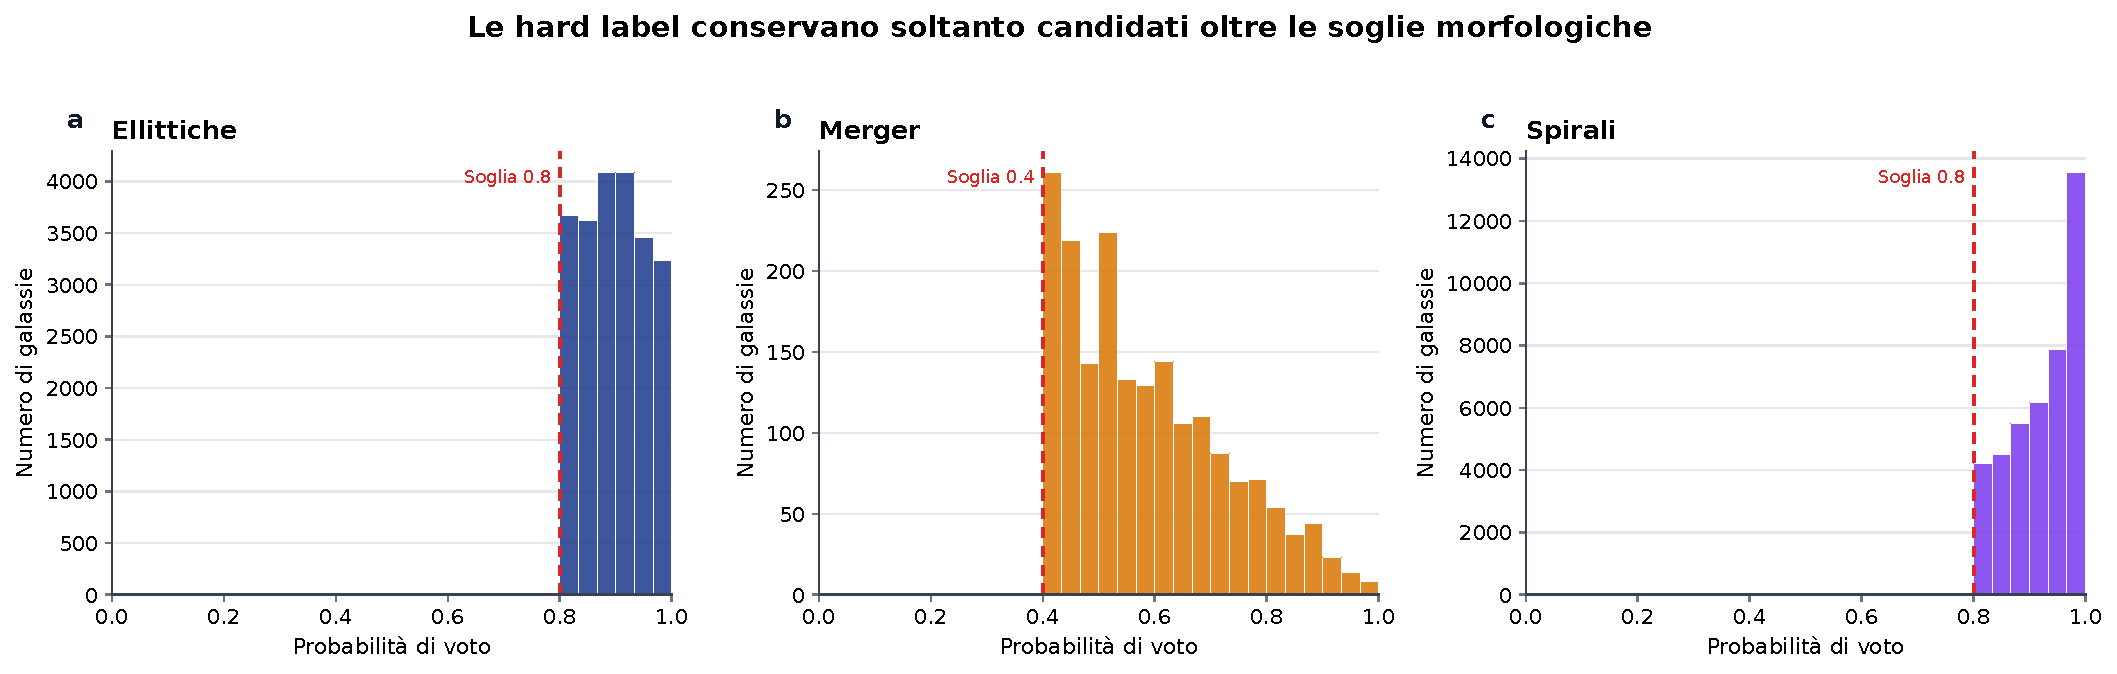
\includegraphics[width=\textwidth]{03_vote_fractions.pdf}
\caption{Distribuzione degli indicatori morfologici nei candidati
selezionati, separati secondo la classe assegnata. Le linee verticali
indicano le soglie operative: \(0{,}8\) per ellittiche e spirali,
\(0{,}4\) per merger. Le distribuzioni sono già condizionate dalla
selezione e non rappresentano l'intero catalogo sorgente.}
\label{fig:voti}
\end{figure}

\section{Pulizia, acquisizione e bilanciamento}
\label{sec:pulizia}

\subsection{Integrità del catalogo}

Il catalogo esportato contiene \(65\,906\) righe. La pulizia rimuove
cinque duplicati esatti e \(72\) righe associate a \(36\) identificativi
discordanti. Per questi ultimi vengono escluse tutte le occorrenze,
anziché scegliere arbitrariamente una delle versioni. Rimangono
\(65\,829\) candidati: \(22\,163\) ellittiche, \(1\,877\) merger e
\(41\,789\) spirali.

Gli identificativi SDSS \texttt{objid} vengono conservati come stringhe.
Questa scelta evita gli arrotondamenti che possono essere introdotti
dalla conversione in numeri a virgola mobile di identificativi con molte
cifre. L'identificativo viene usato come chiave nei manifest, nelle
partizioni e nelle predizioni: una sua alterazione comprometterebbe sia
la tracciabilità sia i controlli di sovrapposizione.

\subsection{Pool di acquisizione e controlli sulle immagini}

La classe merger, con \(1\,877\) candidati, determina la scala del
bilanciamento. Per disporre di una riserva in caso di download non riusciti
o immagini non valide, il pool di acquisizione comprende tutti i merger
e \(2\,347\) oggetti per ciascuna delle altre due classi:
\[
  2\,347=\left\lceil 1{,}25\cdot1\,877\right\rceil.
\]
Il campionamento utilizza il seed di progetto \(42\). Il pool contiene
complessivamente \(6\,571\) oggetti, senza richiedere il download di
tutti i candidati del catalogo.

Per ogni oggetto viene richiesto al servizio SDSS un ritaglio
(\emph{cutout}) JPEG RGB di \(320\times320\) pixel, centrato sulle
coordinate catalogate, con scala di \(0{,}396\) secondi d'arco per pixel.
Il lato dell'immagine corrisponde quindi a circa \(126{,}7\) secondi
d'arco. Si tratta di immagini di visualizzazione a colori, non di un
addestramento direttamente sui dati fotometrici grezzi delle singole bande.

La validazione verifica leggibilità e integrità del file, dimensioni,
modalità RGB, dimensione minima di \(512\) byte e variabilità della
luminanza. Quest'ultima è calcolata dai canali RGB tramite
\[
  Y=0{,}2126R+0{,}7152G+0{,}0722B;
\]
è richiesta una deviazione standard di almeno \(1\), sulla scala
\(0\)--\(255\), per individuare immagini sostanzialmente uniformi.
Tutti i \(6\,571\) cutout del pool superano i controlli.

Viene inoltre calcolata l'impronta SHA-256 dei file per rilevare
duplicati identici a livello di byte, sia entro una classe sia tra
classi diverse. Nel pool validato non emergono duplicati di questo tipo.
Il controllo non equivale tuttavia a una deduplicazione percettiva:
due immagini dello stesso sistema con ritagli o codifiche differenti
possono avere hash diversi. Analogamente, identificativi distinti non
garantiscono che due cutout non includano porzioni di cielo comuni.

\subsection{Dataset finale}

Il numero finale per classe è fissato a \(1\,876\), arrotondando
\(1\,877\) al multiplo di quattro inferiore. Questo consente quote
stratificate esatte per la successiva ripartizione \(50/25/25\).
Il campionamento finale è deterministico e usa il seed di progetto con
un offset dipendente dalla classe.

La \cref{tab:dataset-numeri} e la \cref{fig:attrition} riepilogano le
numerosità. Dei \(6\,571\) file validi, \(943\) non entrano nel campione
finale: \(471\) ellittiche, un merger e \(471\) spirali. Queste esclusioni
derivano dal bilanciamento e non da un fallimento dei controlli di qualità.

\begin{table}[tbp]
\centering
\caption{Numerosità nelle principali fasi della costruzione del dataset.
Il pool validato coincide con quello acquisito; il passaggio finale
riduce il campione per bilanciamento.}
\label{tab:dataset-numeri}
\begin{tabular}{lrrrr}
\toprule
\rowcolor{ThesisTableHeader}
\tablehead{Fase} & \tablehead{Ellittiche} & \tablehead{Merger} & \tablehead{Spirali} & \tablehead{Totale} \\
\midrule
Candidati puliti & \(22\,163\) & \(1\,877\) & \(41\,789\) & \(65\,829\) \\
Pool acquisito & \(2\,347\) & \(1\,877\) & \(2\,347\) & \(6\,571\) \\
Immagini valide & \(2\,347\) & \(1\,877\) & \(2\,347\) & \(6\,571\) \\
Dataset finale & \(1\,876\) & \(1\,876\) & \(1\,876\) & \(5\,628\) \\
\bottomrule
\end{tabular}
\end{table}

\begin{figure}[tbp]
\centering
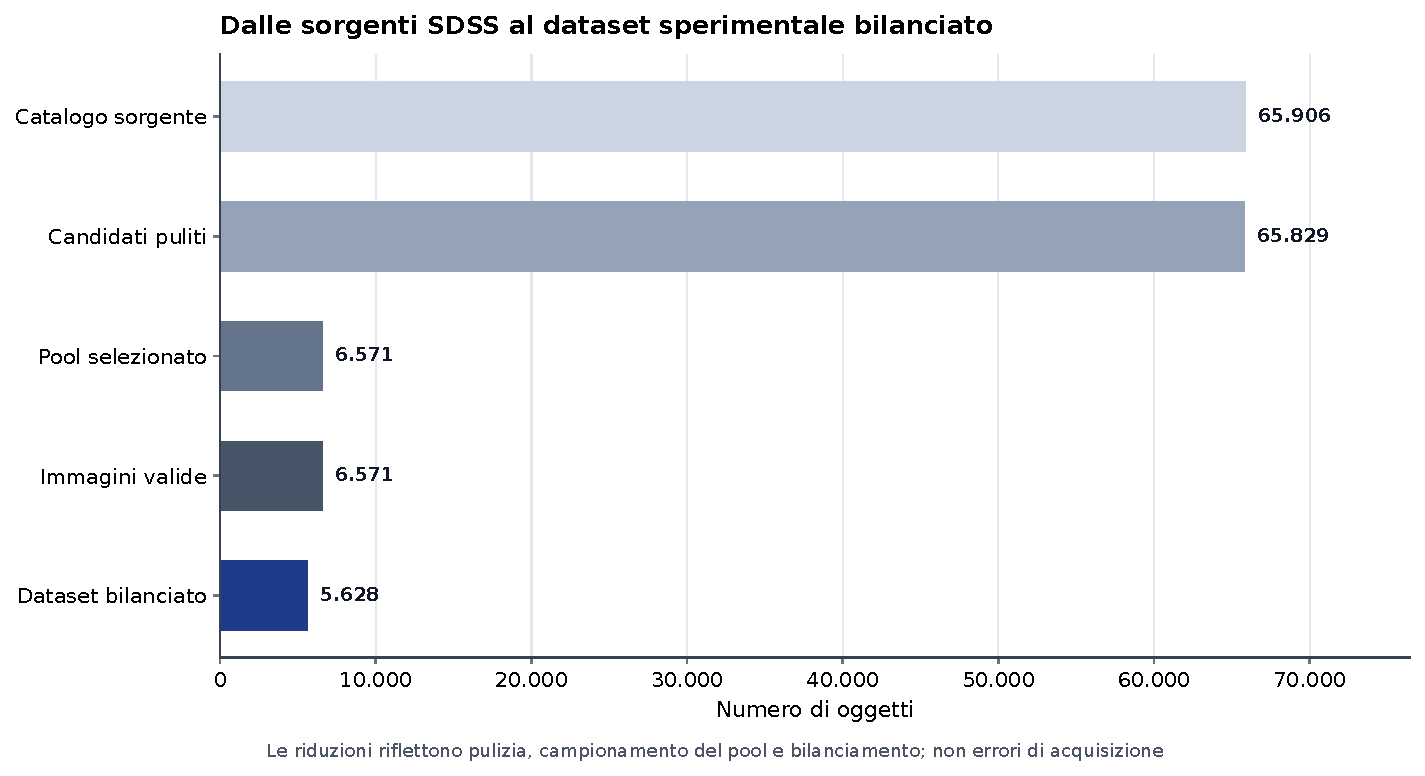
\includegraphics[width=\textwidth]{01_data_attrition.pdf}
\caption{Numerosità lungo la pipeline: catalogo esportato, candidati
puliti, pool di download, immagini valide e dataset finale. La riduzione
tra candidati e pool è una selezione pianificata; quella tra immagini
valide e dataset finale dipende dal bilanciamento.}
\label{fig:attrition}
\end{figure}

Il cambiamento della composizione di classe è illustrato nella
\cref{fig:bilanciamento}. Il bilanciamento facilita il confronto tra
classi e impedisce che la numerosità molto maggiore delle spirali
domini l'addestramento. Modifica però la prevalenza rispetto al catalogo:
metriche aggregate e probabilità prodotte dal classificatore non possono
essere trasferite automaticamente a una popolazione astronomica con
frequenze diverse.

\begin{figure}[tbp]
\centering
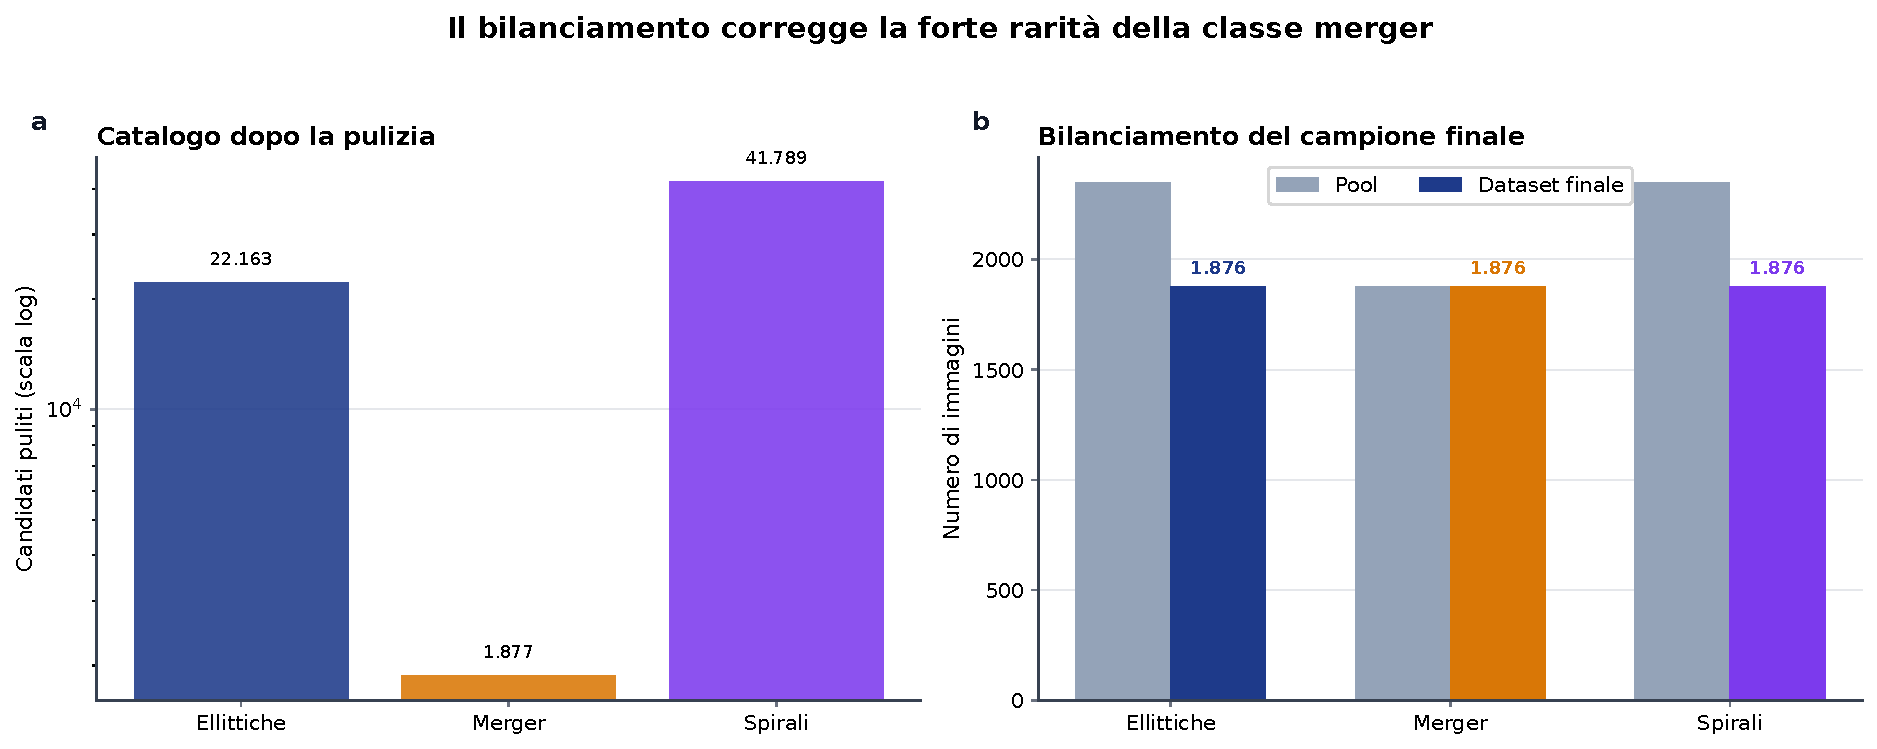
\includegraphics[width=\textwidth]{02_class_balance.pdf}
\caption{Composizione per classe dei candidati, del pool di acquisizione
e del dataset finale. Il pannello dei candidati utilizza una scala
logaritmica. Il campione finale contiene \(1\,876\) oggetti per classe;
questa distribuzione è una scelta sperimentale, non una stima della
prevalenza delle morfologie nella popolazione SDSS.}
\label{fig:bilanciamento}
\end{figure}

\section{Caratteristiche del campione e trasformazioni}
\label{sec:trasformazioni}

\subsection{Redshift e limiti del controllo osservativo}

La \cref{fig:redshift} descrive il redshift delle tre classi nel dataset
finale. Il bilanciamento numerico non rende identiche le distribuzioni
delle altre proprietà: le classi mantengono distribuzioni di redshift
differenti. La figura è una descrizione del campione, non un test di
significatività né una dimostrazione che il redshift causi gli errori
del classificatore.

\begin{figure}[tbp]
\centering
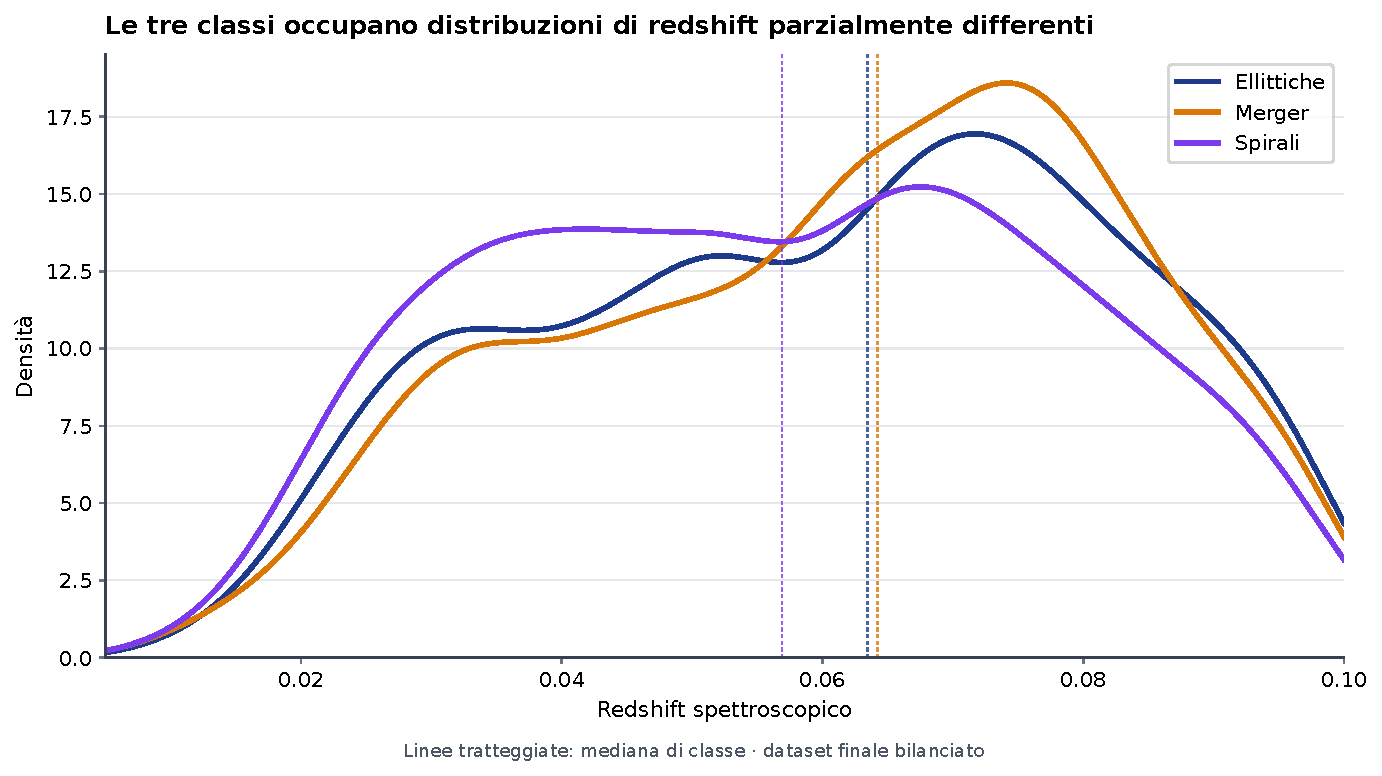
\includegraphics[width=\textwidth]{04_redshift_distribution.pdf}
\caption{Distribuzione del redshift nel dataset finale, distinta per
classe. Le curve rappresentano stime di densità; le linee verticali
indicano le mediane. La selezione nell'intervallo
\(0{,}005<z<0{,}1\) non comporta un abbinamento delle distribuzioni di
redshift tra classi.}
\label{fig:redshift}
\end{figure}

Coordinate, redshift e frazioni di voto sono usati per costruzione e audit
del dataset, non come input aggiuntivi del classificatore. Ciò non esclude
che proprietà correlate a questi metadati, come dimensione apparente o
risoluzione delle strutture, siano presenti nelle immagini. Non è stato
applicato un abbinamento tra classi per redshift o dimensione angolare.
Questo aspetto delimita l'interpretazione astronomica dei risultati.

\subsection{Preprocessing e rappresentazione condivisa}

Le immagini di training sono ruotate di un angolo casuale tra
\(0^\circ\) e \(360^\circ\), con interpolazione bilineare, quindi
ritagliate centralmente a \(224\times224\) pixel. Seguono riflessioni
orizzontali e verticali, ciascuna con probabilità \(0{,}5\).
Il ritaglio viene effettuato dopo la rotazione: il buffer iniziale
da \(320\) pixel consente di mantenere il quadrato centrale senza i bordi
neri introdotti agli angoli. In particolare,
\(320/\sqrt{2}\simeq226{,}3>224\).

I valori vengono convertiti in tensori e normalizzati per canale con
medie \((0{,}485,0{,}456,0{,}406)\) e deviazioni standard
\((0{,}229,0{,}224,0{,}225)\), coerentemente con i pesi ImageNet
utilizzati. Validation e test impiegano soltanto ritaglio centrale,
conversione e normalizzazione, senza trasformazioni casuali.

Le immagini così trasformate sono elaborate da una ResNet18
\cite{he2016resnet} con pesi \texttt{IMAGENET1K\_V1} di
TorchVision~\cite{torchvisionresnet18}. Il classificatore finale viene
rimosso e ogni immagine è rappresentata da un vettore di \(512\) feature.
Il backbone è congelato e utilizzato in modalità di valutazione:
l'esperimento confronta pertanto classificatori che ricevono una
rappresentazione classica condivisa, non backbone addestrati separatamente.

Le feature sono precalcolate e conservate in una cache per ripetizione.
Nella procedura utilizzata, l'augmentation del training produce una
vista per oggetto al momento della costruzione della cache: tale vista
rimane fissa nelle epoche successive. Non si tratta quindi di una nuova
rotazione a ogni epoca. La condivisione della cache mantiene costante
anche questa componente del confronto tra modelli. Il dettaglio delle
teste classiche e quantistiche è rinviato al \cref{chap:modelli}.

\section{Task e repeated holdout stratificato}
\label{sec:holdout}

Il task a tre classi utilizza tutte le immagini del dataset finale.
Il task binario considera soltanto ellittiche e spirali, escludendo
i merger e rimappando le etichette a due classi. Le partizioni binarie
derivano dal filtraggio delle corrispondenti partizioni a tre classi:
gli oggetti delle due classi comuni mantengono dunque il proprio ruolo
di training, validation o test nella stessa ripetizione.

Per ciascun repeat seed il campione viene suddiviso in tre insiemi
disgiunti: \(50\%\) per l'addestramento, \(25\%\) per la validazione e
\(25\%\) per il test. La stratificazione preserva il bilanciamento
tra classi in ogni insieme. Le numerosità sono riportate nella
\cref{tab:split}.

\begin{table}[tbp]
\centering
\caption{Numerosità per ciascuna ripetizione del protocollo.
Nella riga per classe i conteggi valgono per ciascuna classe presente
nel task. La denominazione \texttt{full} indica la colonna Training.}
\label{tab:split}
\begin{tabular}{lrrrr}
\toprule
\rowcolor{ThesisTableHeader}
\tablehead{Task} & \tablehead{Training} & \tablehead{Validation} & \tablehead{Test} & \tablehead{Totale} \\
\midrule
Binario & \(1\,876\) & \(938\) & \(938\) & \(3\,752\) \\
Tre classi & \(2\,814\) & \(1\,407\) & \(1\,407\) & \(5\,628\) \\
Per classe & \(938\) & \(469\) & \(469\) & \(1\,876\) \\
\bottomrule
\end{tabular}
\end{table}

I dieci repeat seed utilizzati sono
\[
  42,\;314,\;2718,\;1618,\;2026,\;7,\;73,\;137,\;1729,\;4096.
\]
Ogni seed definisce una ripetizione riproducibile. Tutti i modelli
condividono le stesse partizioni all'interno della ripetizione: il
confronto delle prestazioni viene così effettuato sugli stessi oggetti
di test e con gli stessi dati disponibili per l'apprendimento.

L'implementazione costruisce quattro blocchi stratificati di uguale
dimensione, con mescolamento determinato dal seed, e ne assegna due al
training, uno alla validation e uno al test. L'esperimento conserva
esclusivamente la prima assegnazione, identificata negli artefatti da
\texttt{iteration=1}. Le altre rotazioni non contribuiscono ai risultati
della tesi. Il protocollo effettivamente valutato è quindi un
\emph{repeated holdout stratificato}, non una cross-validation completa
a quattro fold.

La validation è impiegata per monitorare l'apprendimento e selezionare
il checkpoint secondo il criterio definito nel
\cref{chap:modelli}; il test è riservato alla valutazione del modello
selezionato. La separazione tra questi ruoli evita che il test venga
usato come criterio operativo di arresto dell'addestramento.

La disgiunzione vale entro ciascuna ripetizione. Tra ripetizioni diverse
uno stesso oggetto può invece comparire più volte nel test, oppure
cambiare ruolo. I dieci risultati misurano quindi la variabilità del
protocollo sul medesimo dataset, non quella di dieci campioni astronomici
indipendenti. Questa dipendenza va tenuta presente nell'interpretazione
degli intervalli e impedisce di trattare tutte le predizioni concatenate
come osservazioni indipendenti.

\section{Regimi a ridotta disponibilità di dati}
\label{sec:subset}

Per studiare il comportamento in condizioni \emph{low-resource}, il
training set viene ridotto a \(100\), \(300\) e \(900\) immagini
complessive. Il numero indica il totale del sottoinsieme, non il numero
per classe. Validation e test restano invariati rispetto alla
ripetizione \texttt{full}: una variazione delle prestazioni non dipende
quindi dalla sostituzione del campione su cui vengono misurate.

La selezione è bilanciata, salvo gli inevitabili arrotondamenti.
Nel task binario i tre regimi contengono rispettivamente \(50\), \(150\)
e \(450\) immagini per classe; nel task a tre classi, il regime da
\(100\) immagini contiene \(33\), \(33\) e \(34\) esempi, mentre quelli
da \(300\) e \(900\) ne contengono rispettivamente \(100\) e \(300\)
per classe.

Per ciascuna combinazione di task e repeat seed, ogni sottoinsieme
è selezionato esclusivamente dal training completo:
\begin{equation}
  \mathcal{T}_{n}^{(s)}\subset\mathcal{T}_{\mathrm{full}}^{(s)},
  \qquad n\in\{100,300,900\}.
  \label{eq:subset-training}
\end{equation}
La selezione usa un seed condiviso tra i modelli:
un controllo classico e il corrispondente classificatore quantistico
non vengono addestrati su campioni estratti separatamente.

Il \cref{lst:training-subset} riporta il nucleo di
\texttt{select\_training\_subset}, in \texttt{scripts/train.py},
con i ritorni a capo adattati. Sono omessi import, gestione del regime
Full e costruzione del contenitore di uscita. La selezione avviene per
identificativo di oggetto, non per singola vista aumentata.

\begin{code}
\begin{minted}{python}
requested = int(subset_size)
identities = bank.metadata[["objid", "label"]].drop_duplicates("objid")
if requested >= len(identities):
    return bank
selected, _ = train_test_split(
    identities, train_size=requested,
    stratify=identities["label"], random_state=seed
)
mask = bank.metadata["objid"].isin(selected["objid"])
metadata = bank.metadata.loc[mask].reset_index(drop=True).copy()
features = bank.features[torch.from_numpy(mask.to_numpy())]
metadata["feature_index"] = range(len(metadata))
\end{minted}
\caption{Selezione stratificata dei soli dati di training.}
\label{lst:training-subset}
\end{code}

Nel notebook di esecuzione dei subset, il seed di selezione è quello
\texttt{dataloader}, condiviso dalle architetture. Il codice conservato
effettua una chiamata separata per ciascuna numerosità: non impone
esplicitamente l'inclusione del campione da 100 in quello da 300 e
di quest'ultimo in quello da 900. Inoltre, il riepilogo denominato
\texttt{nested\_audit} registra le numerosità, ma non verifica tali
inclusioni. Non si assume pertanto un annidamento reciproco dimostrato.
Le curve descrivono l'effetto del regime di campionamento; le differenze
possono dipendere anche dalla composizione del sottoinsieme, oltre che
dalla numerosità e dalla variabilità dell'ottimizzazione.

Il regime \texttt{full} corrisponde a \(1\,876\) immagini di training nel
binario e a \(2\,814\) nel task a tre classi. Nei grafici comparativi
questa etichetta deve dunque essere distinta da una numerosità universale.
Le curve rispetto a \(100\), \(300\), \(900\) e \texttt{full} descrivono
l'effetto della quantità di dati, non l'andamento della loss nelle epoche.

\section{Tracciabilità e perimetro delle conclusioni}
\label{sec:tracciabilita}

La pipeline conserva manifest del catalogo, download, validazione e
campione finale, insieme alle assegnazioni dei singoli oggetti alle
partizioni. Gli artefatti di ogni run comprendono configurazione,
cronologia dell'addestramento, checkpoint, metriche e predizioni.
Il collegamento tramite identificativi consente di ricondurre una metrica
aggregata agli esempi valutati e di verificare l'appaiamento tra modelli.

Ai fini del confronto sperimentale, i principali controlli sono
l'unicità degli identificativi nel campione, la verifica degli hash,
la separazione dei ruoli entro ciascun holdout, la condivisione delle
feature e l'invarianza di validation e test nei regimi ridotti.
Questi controlli non sostituiscono una validazione esterna. Rimangono
possibili rumore nelle etichette, differenze osservazionali tra classi
e correlazioni tra oggetti astronomicamente vicini; non viene effettuata
una suddivisione per gruppi di sistemi fisici o regioni di cielo.

Il protocollo consente pertanto di studiare l'effetto della scelta del
classificatore su una rappresentazione e su partizioni controllate.
Non misura, da solo, la capacità di generalizzare a survey differenti
o a una popolazione con diversa prevalenza morfologica. Su questa base,
il capitolo successivo definisce le architetture, le condizioni di
addestramento e i confronti statistici con cui vengono valutate le
domande di ricerca.
